\documentclass{beamer} 
\usepackage[utf8]{inputenc}
\usepackage{polski}
\usepackage{tikz}

\usetheme{Copenhagen}

\author[]{Paweł Koniszewski \\ Przemysław Kubicki \\ Tomasz Wesołowski}

\institute[Politechnika Gdańska, ETI]{Politechnika Gdańska, Wydział Elektrotechniki, Telekomunikacji i Informatyki}
\date{Gdańsk, \today}
\title[Armadio]{Program rozszerzonej rzeczywistości do meblowania pomieszczeń \\ ARMADIO}

\newtheorem{dfn}{Definicja}
\begin{document}

\frame{\titlepage}

\frame{
	\frametitle{Agenda}
	\tableofcontents
}

\section{Rozszerzona rzeczywistość}

\frame{
	\tableofcontents[currentsection]
}

\subsection{Definicja}
\frame{
	\frametitle{Definicja}
	\begin{dfn}
	Rzeczywistość wirtualna stworzona z połączenia prawdziwego i wirtualnego świata
	\end{dfn}
	\begin{dfn}
Ronald Azuma zdefiniował rozszerzoną rzeczywistość jako:
	\begin{itemize}
		\item łączącą w sobie świat realny oraz rzeczywistość wirtualną
		\item interaktywną w czasie rzeczywistym
		\item umożliwiającą swobodę ruchów w trzech wymiarach
	\end{itemize}
	\end{dfn}
}
	
\subsection{Zastosowania}
\frame{
	\frametitle{Niektóre z zastosowań}
	Branże:
	\begin{itemize}
		\item marketing
		\item edukacja
		\item medycyna
		\item lotnictwo
		\item \ldots
	\end{itemize}
}

\frame{
	\frametitle{Niektóre z zastosowań}
	Szczegółowe:
	\begin{itemize}
		\item Gry planszowe
		\item Instrukcje obługi
		\item Portale społecznościowe
		\item \ldots
	\end{itemize}
}

\subsection{Przykłady}
\frame{
	\frametitle{Przykłady}
	\begin{itemize}
	\item Google glass
	\item Layar, Wikitude
	\item Filmy ("Raport mniejszości", "Ironman", \ldots)
	\item Gry ("ArDefender", \ldots)
	\end{itemize}
}

\section{Geneza tematu}

\frame{
	\tableofcontents[currentsection]
}

\subsection{Klasyczne aplikacje}
\frame{
	\frametitle{Klasyczne aplikacje - dla profesjonalistów}
	Profesjonalne aplikacje:
	\begin{itemize}
	\item{AutoCAD}
	\item{IntelliCAD}
	\item{VariCAD}
	\item{TurboCAD}
	\end{itemize}
}

\frame{
	\frametitle{Klasyczne aplikacje - dla amatorów}
	Aplikacje dla amatorów:
	\begin{itemize}
	\item{Furnish}
	\item{Home Planner}
	\item{Power NET+}
	\item{Light Decor Paradyż}
	\end{itemize}
}

\frame{
	\frametitle{Klasyczne aplikacje - przykłady}
            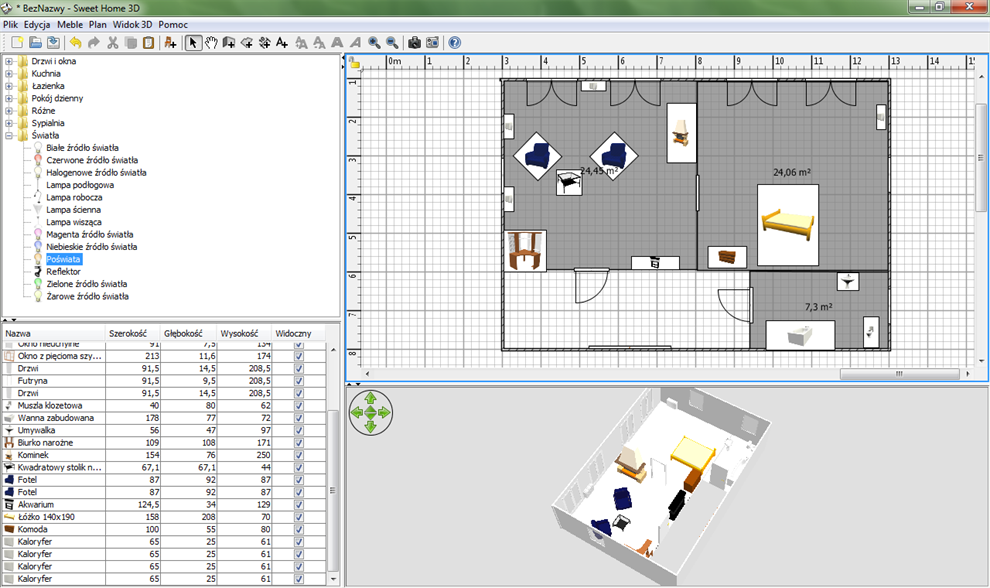
\includegraphics[width=300pt]{img/sweet_home.png}
}

\frame{
	\frametitle{Klasyczne aplikacje - przykłady}
           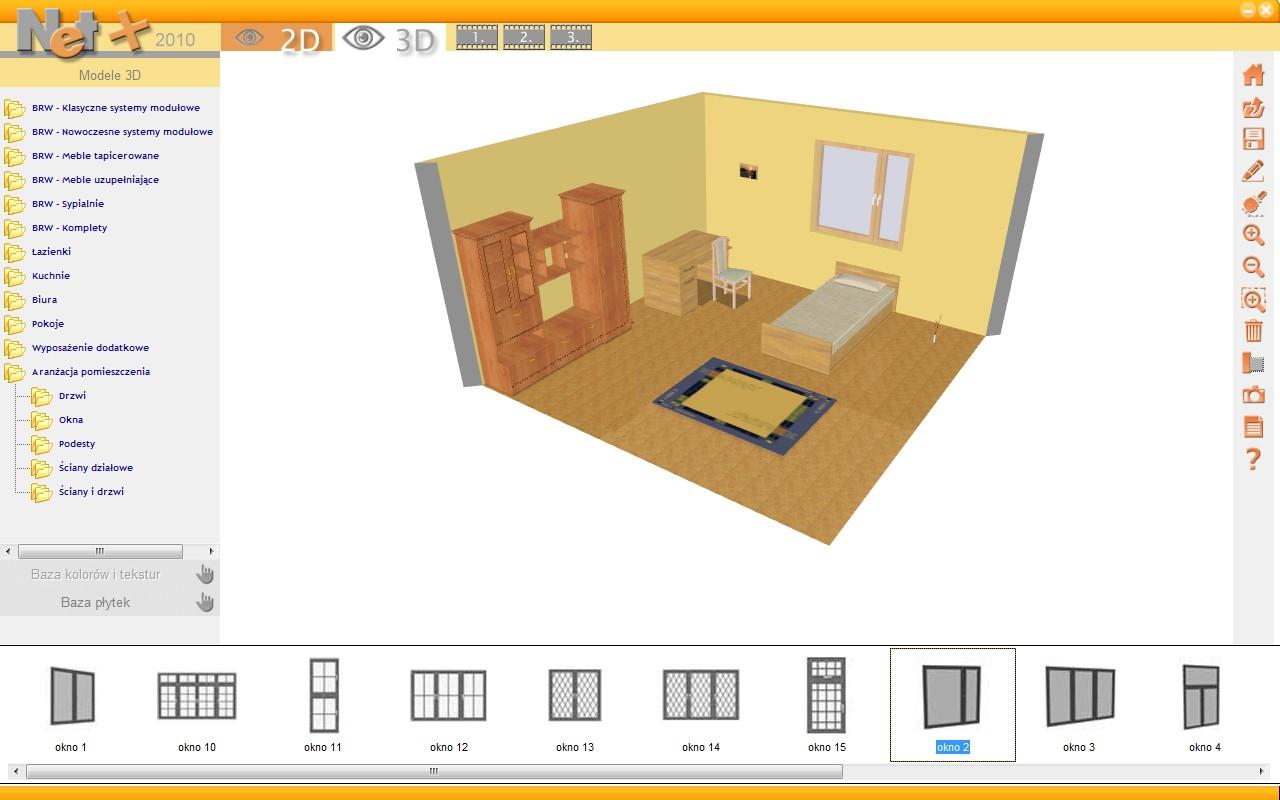
\includegraphics[width=300pt]{img/net_plus.jpg}

}

\subsection{Aplikacje rozszerzonej rzeczywistości}
\frame{
	\frametitle{Rozwiązania mobilne}
	Aplikacje na smartphone'y:
	\begin{itemize}
	\item{ViewAR}
	\item{???}
	\end{itemize}
}

\section{Armadio}

\frame{
	\tableofcontents[currentsection]
}

\subsection{Cele}
\frame{
	\frametitle{Cele aplikacji}
	\begin{minipage}[t]{0.48\linewidth}
		Główne cele:
		\begin{itemize}
		\item{Jeden marker - wiele mebli}
		\item{Ingerencja w modele}
		\item{Wykorzystanie czujników}
		\end{itemize}
	\end{minipage}\hfill
	\begin{minipage}[t]{0.48\linewidth}
		Cele poboczne:
		\begin{itemize}
		\item{Możliwość dogrania własnych modeli}
		\item{Zdalne doczytywanie modeli}
		\end{itemize}
	\end{minipage}
}

\subsection{Biblioteki i środowisko - research}
\frame{}

\frame{
	\frametitle{Środowisko pracy - Unity}
	\begin{dfn}
	$\mathbf{Unity}$ - zintegrowane narzędzie do tworzenia gier trójwymiarowych lub innych materiałów interaktywnych
	\end{dfn}
	$\mathbf{Cechy:}$
	\begin{itemize}
	\item fajne
	\item multiplatformowość
	\item multijęzykowość
	\item darmowe
	\end{itemize}
}

\subsection{Technologie}
\frame{

}

\subsection{Postęp prac}
\frame{
	\frametitle{Postęp prac}

}

\subsection{TODO}
\frame{
	\frametitle{Do zrobienia}
	
}

\subsection{Prezentacja aplikacji}
\frame{
	\frametitle{Prezentacja ARmadio}
	
}


\frame{
	Dziękujemy za uwagę.
}

\end{document}